\section{Integration}
\subsection{The Riemann Integral}
Our goal is the following: for a ``sufficiently nice'' function $f:[a,b]\to\mathbb R$ we want to define its integral
$$\int_a^bf(x)\,\mathrm dx$$
We would like to think of this as the area under the graph of $y=f(x)$, which motivates the Riemann integral.
\begin{definition}
    $f:[a,b]\to \mathbb{R}$ is called \textbf{bounded} if $ \exists K,\ \forall x\in [a,b],\ |f(x)|\le K $. 
\end{definition}
\begin{definition}
    A dissection(or partition) of the interval $[a,b]$ is a finite subset $D\subseteq [a,b]$ such that $a,b\in D$.
    If $D$ is a dissection, we can write $D=\{a_0,\ldots,a_n\}$ where $a=a_0<a_1<\cdots<a_n=b$.
\end{definition}
Note that if $D,D'$ are both dissections, so is $D\cup D'$.
\begin{definition}
    If $f:[a,b]\to\mathbb R$ is bounded and a dissection $D$ consists of $a=a_0<a_1<\cdots<a_n=b$, then we define the \textbf{upper} and \textbf{lower} \textbf{Riemann sums} wrt $D$ by
    respectively.
    \begin{align*}
        U(f,D)&=\sum_{i=1}^n(a_i-a_{i-1})\sup_{x\in [a_{i-1},a_i]}f(x),\\ 
        L(f,D)&=\sum_{i=1}^n(a_i-a_{i-1})\inf_{x\in [a_{i-1},a_i]}f(x).
    \end{align*}
    They exists as $f$ is bounded.
\end{definition}
Clearly $ L(f,D)\le U(f,D),\ \forall D $.
\begin{lemma}\label{lma:5.1}
    If $D\subseteq D'$ are dissections of $[a,b]$, then 
    \[
        U(f,D)\ge U(f,D')\ge L(f,D')\ge L(f,D).
    \]
\end{lemma}
\begin{proof}
    $U(f,D')\ge L(f,D')$ is obvious. Suppose $ D' $ contains an extra point than $D$, say $ y\in (x_{r-1},x_r) $. Clearly 
    \[
        \sup_{x\in [x_{r-1},y]}f(x),\sup_{x\in [y,x_r]}f(x)\le \sup_{x\in [x_{r-1},x_r]}f(x),
    \]
    so 
    \[
        (x_r-x_{r-1})\sup_{x\in [x_{r-1},x_r]}f(x)\ge (y-x_{r-1})\sup_{x\in [x_{r-1},y]}f(x)+(x_r-y)\sup_{x\in [y,x_r]}f(x).
    \]
    Summing over gives the result. Similarly for $D'$ with more extra points and $ L $.
\end{proof}
\begin{lemma}
    If $D_1,D_2$ are dissections of $[a,b]$, then
    \[
        U(f,D_1)\ge U(f,D_1 \cup D_2)\ge L(f,D_1 \cup D_2)\ge L(f,D_2).
    \]
\end{lemma}
\begin{proof}
    Take $ D'=D_1 \cup D_2 $ in the previous lemma.
\end{proof}

\begin{definition}
    The \textbf{upper integral} of $f$ is defined as 
    \[
        U(f) = \inf_D U(f,D),
    \]
    and the \textbf{lower integral} of $f$ is defined as 
    \[
        L(f) = \sup_D L(f,D).
    \]
    They both exists since $ U(f,D),L(f,D) $ are bounded.
\end{definition}
Hence 
\begin{sprop}
    $U(f)\ge L(f)$.
\end{sprop}

\begin{definition}
    A bounded function $ f:[a,b]\to \mathbb{R}  $ is said to be \textbf{Riemann integrable} on $[a,b]$ if $ U(f)=L(f) $ and we set
    $$\int_a^bf(x)\,\mathrm dx=L(f)=U(f) = \int_{a}^{b} f.$$
\end{definition}
\begin{example}\
    \begin{enumerate}
        \item Consider $f(x)=c$ for a constant $c$ for all $x\in [a,b]$, then consider $D=\{a,b\}$, then $U(f,D)=c(b-a)=L(f,D)$, hence $U(f)=c(b-a)=L(f)$, therefore $f$ is Riemann integrable and
        $$\int_a^bf(x)\,\mathrm dx=c(b-a).$$
        \item $f:[a,b]\to\mathbb R$ by $f(x)=0$ if $x\in\mathbb Q$ and $f(x)=1$ if $x\in\mathbb R\setminus\mathbb Q$. Note that if $a_{i-1}<a_i$, then $[a_{i-1},a_i]$ contains both rational and irrational numbers, so it follows that $U(f,D)=b-a$ and $L(f,D)=0$ for any dissection $D$ of $[a,b]$, therefore $U(f)=b-a\neq 0=L(f)$, hence $f$ is not Riemann integrable.
    \end{enumerate}
\end{example}

\subsection{Properties of riemann integrals}
\begin{theorem}\label{thm:5.3}
    Bounded $f:[a,b]\to\mathbb R$ is Riemann integrable on $[a,b]$ if and only if for every $\epsilon>0$, there is a dissection $D$ of $[a,b]$ such that 
    \[
        U(f,D)-L(f,D)<\epsilon.
    \]
\end{theorem}
\begin{proof}
    For every dissection $ D $ we have 
    \[
        0\le U(f)-L(f)\le U(f,D)-L(f,D).
    \]
    If the given condition holds, then 
    \[
        0\le U(f)-L(f)\le U(f,D)-L(f,D)<\epsilon,\quad \forall \epsilon>0.
    \]
    Immediately, $ L(f)=U(f) $.

    Suppose conversely $ f $ is integrable, by definition of $ \sup ,\inf  $, $ \exists D_1,D_2 $ such that 
    \begin{align*}
        &\int_{a}^{b} f(x) \,\mathrm{d}x -\frac{\epsilon}{2} = L(f)-\frac{\epsilon}{2} < L(f,D_1),\\ 
        &U(f,D_2)<U(f)+\frac{\epsilon}{2}=\int_{a}^{b} f(x) \,\mathrm{d}x+\frac{\epsilon}{2}.
    \end{align*}
    By lemma \ref{lma:5.1}, 
    \[
        U(f,D_1 \cup D_2)-L(f,D_1 \cup D_2)\le U(f,D_2)-L(f,D_1)<\epsilon.
    \]
\end{proof}
\begin{theorem}\label{thm:5.4}
    If $ f:[a,b]\to \mathbb{R} $ is monotonic, then $f$ is integrable.
\end{theorem}
\begin{proof}
    Wlog suppose $ f \nearrow $. Then
    \[
        \sup_{x\in [x_{j-1},x_j]}f(x)=f(x_j)\quad \text{and}\quad \inf_{x\in [x_{j-1},x_j]}f(x)=f(x_{j-1}).
    \]
    Thus 
    \[
        U(f,D)-L(f,D) = \sum_{j=1}^{n}(x_j-x_{j-1})[f(x_j)-f(x_{j-1})].
    \]
    Now consider 
    \[
        D = \left\{ a,a+\frac{b-a}{n},\dots,b \right\}.
    \]
    We have 
    \[
        U(f,D)-L(f,D)=\frac{b-a}{n}(f(b)-f(a)).
    \]
    Take $n$ large enough so that $ U(f,D)-L(f,D)<\epsilon $, and use theorem \ref{thm:5.3}
\end{proof}
\begin{definition}[Uniform continuity]
    $ f:[a,b]\to \mathbb{R} $ is called \textbf{uniformly continuous} if $ \forall \epsilon>0,\ \exists \delta>0,\ \forall x,y\in [a,b],\ |x-y|<\delta \Rightarrow |f(x)-f(y)|<\epsilon $.
\end{definition}
\begin{lemma}\label{lma:5.5}
    If $ f:[a,b]\to \mathbb{R}  $ is continuous, then it is uniformly continuous.
\end{lemma}
\begin{proof}[Proof by contradiction.]
    Suppose the claim is false. Then $ \exists \epsilon>0,\ \forall \delta>0,\ \exists x,y\in [a,b],\ |x-y|<\delta $ but $ |f(x)-f(y)|\ge \epsilon $. Take $ \delta=1/n $ to get $ x_n,y_n $ with such property. By Bolzano-Weierstrass, $ \exists x_{n_k}\to c $. Note that 
    \[
        |y_{n_k}-c|\le |y_{n_k}-x_{n_k}|+|x_{n_k}-c|\to 0 \Longleftrightarrow y_{n_k}\to c,
    \]
    but $ |f(x_{n_k})-f(y_{n_k})|\ge \epsilon $. Let $ k\to \infty $, by continuity, $ |f(x_{n_k})-f(y_{n_k})|\to 0 $, \#.
\end{proof}

\begin{theorem}\label{thm:5.6}
    Let $f:[a,b]\to \mathbb{R}$ be continuous, then $f$ is integrable. 
\end{theorem}
\begin{proof}
    By lemma, $ \forall \epsilon>0,\ \exists \delta>0,\ \forall x,y\in [a,b],\ |x-y|<\delta \Rightarrow |f(x)-f(y)|<\epsilon $. Let 
    \[
        D=\left\{ a+\frac{(b-a)j}{n}:j=0,\dots,n \right\}.
    \]
    Choose $n$ large so that $ (b-a)/n<\delta $. Then $\forall  x,y\in [x_{j-1},x_j] $, $ |f(x)-f(y)|<\epsilon $. This means that 
    \[
        \max_{x\in [x_{j-1},x_j]}f(x)-\min _{x\in [x_{j-1},x_j]}f(x)=f(p)-f(q),\quad p,q\in[x_{j-1},x_j]
    \]
    by continuity. Now 
    \begin{align*}
        U(f,D)-L(f,D)&= \sum_{j=1}^{n}(x_{j}-x_{j-1})\left( \max_{x\in [x_{j-1},x_j]}f(x)-\min _{x\in [x_{j-1},x_j]}f(x) \right)\\ 
        &= \sum_{j=1}^{n}\frac{(b-a)}{n}(f(p_j)-f(q_j))\\ 
        &<\epsilon(b-a).
    \end{align*}
    Hence $f$ is integrable by theorem \ref{thm:5.3}.
\end{proof}
\begin{example}
    Let $ f:[0,1]\to \bbR $ be defined by 
    \[
        f(x) = \begin{cases}
        1/q & x = p/q \text{ in lowest form}\\
        0 &\text{otherwise}\\
        \end{cases} 
    \]
    Clearly $ L(f,D)=0,\ \forall D $. We will show that $ \forall \epsilon>0,\ \exists D,\ U(f,D)<\epsilon $. This implies $f$ is integrable with 
    \[
        \int_{0}^{1} f(x) \,\mathrm{d}x=0.
    \]
    Take $ N\in \mathbb{N} $ such that $ 1/N<\epsilon/2 $. Consider 
    \[
        \{x\in [0,1]: f(x)\ge 1/N\} = \{p/q:1\le q\le N \land 1\le p\le q\}.
    \]
    This is a finite set with $ 0<t_1<\cdots<t_R=1 $. Consider $D$ such that 
    \begin{enumerate}
        \item Each $ t_k $ is in some interval $ [x_{j-1},x_j] $.
        \item $ \forall k $, the unique interval contaning $t_k$ has length at most $ \epsilon/2. $
    \end{enumerate}
    \begin{center}
        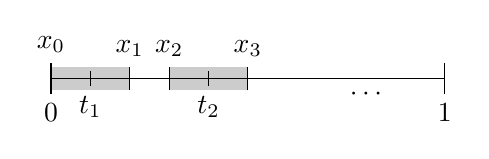
\begin{tikzpicture}
            \fill [black!20] (0,-0.15) rectangle (1,0.15);
            \fill [black!20] (1.5,-0.15) rectangle (2.5,0.15);
            \draw (0,0) -- (5,0);
            \draw (0,-0.2) -- (0,0.2) node [pos=0,below] {$0$} node [pos=1,above] {$x_0$};
            \draw (5,-0.2) -- (5,0.2) node [pos=0,below] {$1$};
            \draw (0.5,-0.1) -- (0.5,0.1) node [pos=0,below] {$t_1$};
            \draw (1,-0.15) -- (1,0.15) node [pos=1,above] {$x_1$};
            \draw (2,-0.1) -- (2,0.1) node [pos=0,below] {$t_2$};
            \draw (1.5,-0.15) -- (1.5,0.15) node [pos=1,above] {$x_2$};
            \draw (2.5,-0.15) -- (2.5,0.15) node [pos=1,above] {$x_3$};
            \node [below] at (4,0) {$ \cdots $};
        \end{tikzpicture}        
    \end{center}
    Outside these intervals, $ f(x)<1/N $. Clearly $ f\le 1 $, so
    \[
        U(f,D)\le 1/N+\frac{\epsilon}{2}<\epsilon.
    \]
\end{example}

\begin{proposition}
    Suppose $f,g:[a,b]\to\mathbb R$ are integrable, then
    \begin{enumerate}
        \item If $\lambda\in\mathbb R$, then $f+\lambda g$ is integrable and
        $$\int_a^bf(x)+\lambda g(x)\,\mathrm dx=\int_a^bf(x)\,\mathrm dx+\lambda\int_a^bg(x)\,\mathrm dx.$$
        \item For any $c\in [a,b]$, $f|_{[a,c]},f|_{[c,b]}$ are integrable and
        $$\int_a^cf(x)\,\mathrm dx+\int_c^bf(x)\,\mathrm dx=\int_a^bf(x)\,\mathrm dx.$$
        \item If $f\ge g$ on $[a,b]$, then
        $$\int_a^bf(x)\,\mathrm dx\ge\int_a^bg(x)\,\mathrm dx.$$
        \item $|f|$ is integrable and
        $$\left|\int_a^bf(x)\,\mathrm dx\right|\le\int_a^b|f(x)|\,\mathrm dx.$$
        \item $fg$ is integrable.
    \end{enumerate}
\end{proposition}
\begin{proof}
    Exercise.
\end{proof}
\begin{notation}
    If $a>b$, let 
    \[
        \int_{a}^{b} f(x) \,\mathrm{d}x = - \int_{b}^{a} f(x) \,\mathrm{d}x
    \]
    and if $a=b$, then let 
    \[
        \int_{a}^{a} f(x) \,\mathrm{d}x=0.
    \]
\end{notation}
With this convention, if $|f|\le K$, then 
\[
    \left| \int_{a}^{b} f(x) \,\mathrm{d}x \right| \le K|b-a|.
\]

\subsection{Fundamental Theorem of Calculus}
Let $f:[a,b]\to \mathbb{R} $ be bounded ($ |f(x)|\le K $) and integrable. Define 
\[
    F(x) = \int_{a}^{x} f(t) \,\mathrm{d}t.
\]
\begin{theorem}\label{thm:5.7}
    $F$ is continuous.
\end{theorem}
\begin{proof}
    Note that 
    \[
        \left| F(x+h)-F(x) \right|  = \left| \int_{x}^{x+h} f(t) \,\mathrm{d}t \right| \le K|h|.
    \]
    let $h\to 0$ gives the result.
\end{proof}

\begin{theorem}[FTC]\label{thm:5.8}
    If $f$ is continuous at $x$, then $F$ is differentiable at $x$ and
    \[
        F'(x)=f(x).
    \] 
\end{theorem}
\begin{proof}
    Need to consider (for $ x+h\in [a,b],h\neq 0 $) that
    \begin{align*}
        \left| \frac{F(x+h)-F(x)}{h}-f(x) \right|&= \frac{1}{|h|}\left| \int_{x}^{x+h} f(t) \,\mathrm{d}t - h f(x) \right| \\ 
        &= \frac{1}{|h|} \left| \int_{x}^{x+h} f(t)-f(x) \,\mathrm{d}t \right| .
    \end{align*}
    Since $f$ is continuous at $x$, given $ \epsilon>0,\ \exists \delta>0  $ such that if $ |t-x|<\delta $, then $ |f(t)-f(x)|<\epsilon$. So if $ |h|<\epsilon $, 
    \[
        \frac{1}{|h|} \left| \int_{x}^{x+h} f(t)-f(x) \,\mathrm{d}t \right|\le \frac{1}{|h|} \epsilon |h| = \epsilon.
    \]
    Which means 
    \[
        \lim_{h \to 0} \frac{F(x+h)-F(x)}{h} = F'(x) = f(x).\qedhere
    \]
\end{proof}
\begin{example}
    Let 
    \[
        f(x) = \begin{cases}
        -1 &x\in [-1,0]\\
        1 &x\in [0,1]\\
        \end{cases} 
    \]
    Check that $f$ is integrable. Check also that $F(x)=-1+|x|$ is differentiable on $ [-1,1]\setminus \{0\} $.
\end{example}
\begin{corollary}[Integration is the inverse of differentiation]
    If $f=g'$ is continuous on $[a,b]$, then 
    \[
        \int_{a}^{x} f(t) \,\mathrm{d}t = g(x)-g(a),\quad \forall x\in [a,b].
    \]
\end{corollary}
\begin{proof}
    By FTC, $(F-g)'=0$ on $ [a,b] $, so it is constant. Since $F(a)=0$, $ F(x)=g(x)-g(a) $ as claimed.
\end{proof}

\begin{note}
    Every continuous function has an \textbf{indefinite integral} or \textbf{anti-derivative} written in 
    \[
        \int f(x) \,\mathrm{d}x
    \]
    which is determined up to a constant.
\end{note}
\begin{remark}
    We actually have solved the ODE 
    \[
        \begin{cases}
         y'(x)=f(x)\\
         y(a)=y_0\\
        \end{cases}
    \]
\end{remark}